\documentclass{article}%
\usepackage[T1]{fontenc}%
\usepackage[utf8]{inputenc}%
\usepackage{lmodern}%
\usepackage{textcomp}%
\usepackage{lastpage}%
\usepackage[head=40pt,margin=0.5in,bottom=0.6in]{geometry}%
\usepackage{graphicx}%
%
\title{\textbf{OVCS: En octubre se registraron 1.418 protestas en el país}}%
\author{EL NACIONAL WEB}%
\date{14/11/2018}%
%
\begin{document}%
\normalsize%
\maketitle%
\textbf{URL: }%
http://www.el{-}nacional.com/noticias/sociedad/ovcs{-}octubre{-}registraron{-}1418{-}protestas{-}pais\_259710\newline%
%
\textbf{Periodico: }%
EN, %
ID: %
259710, %
Seccion: %
Sociedad\newline%
%
\textbf{Palabras Claves: }%
Protestas, Sociedad\newline%
%
\textbf{Derecho: }%
5%
, Otros Derechos: %
NO\_TIENE%
, Sub Derechos: %
NO\_TIENE%
\newline%
%
\textbf{EP: }%
SI\newline%
\newline%
%
\textbf{\textit{En el año 2018 en Venezuela se han documentado un total de 10.733 manifestaciones con diferentes exigencias por parte de los manifestantes}}%
\newline%
\newline%
%
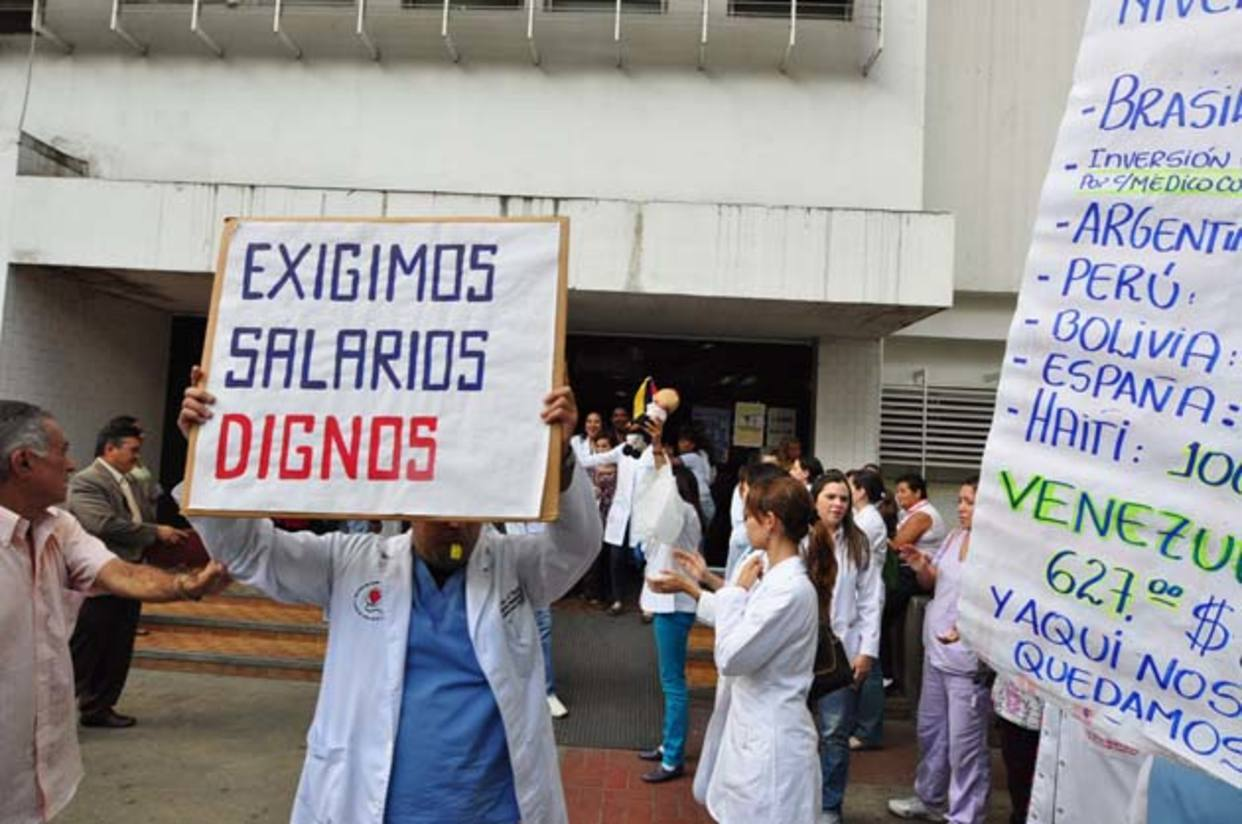
\includegraphics[width=300px]{184.jpg}%
\newline%
%
El Observatorio Venezolano de Conflictividad Social (OVCS), indicó que en octubre del presente año se registraron en el país 1.418 protestas, un total de 47 diarias, lo que suma un total de 10.773 manifestaciones. Lo que representa el mayor número de protestas durante el mandato del presidente Nicolás Maduro.%
\newline%
%
El OVCS informó que en 10 meses la cifra superó las olas de protestas efectuadas en los años 2014 y 2017 en el país, la cuales sumaron 9.286 y 9.787 respectivamente. Lo que representa un incremento de conflictividad de 683\% en comparación a octubre de 2017.%
\newline%
%
Cortesía OVCS%
\newline%
%
En las protestas de octubre se exigieron derechos económicos, sociales, culturales y ambientales (Desca) simultáneamente, El Observatorio estimó que 11\% estuvo relacionada con exigencia de derechos civiles. Durante octubre se realizaron 59 para exigir el derecho a la vida, 49 por justicia y 72 por el ejercicio de derechos políticos. IMAGEN.%
\newline%
%
El OVCS hizo nuevamente un llamado para establecer una agenda en el país en la que se coloque por delante el tema social en vez de priorizar intereses políticos, que afecta el estilo de vida de los venezolanos indistintamente de su afinidad política.%
\newline%
%
Con información del~OVCS%
\newline%
%
\end{document}